\begin{figure}[ht]
	\centering
	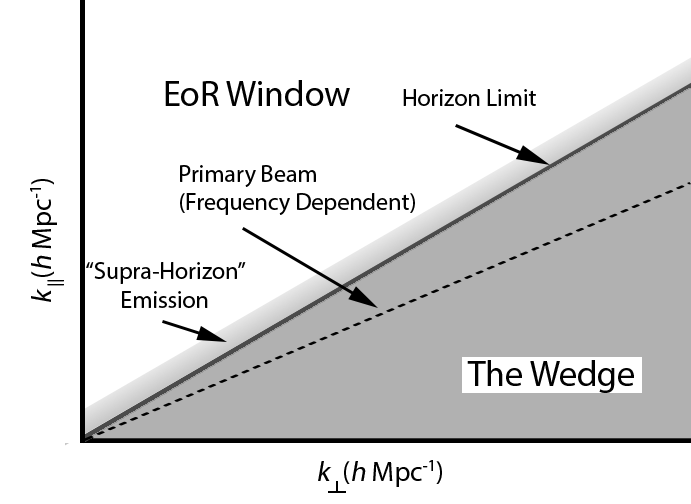
\includegraphics[width=0.75\textwidth]{wedge-diagram.png}
	\caption[Foreground Wedge]{Foreground Wedge}
	\label{fig:wedge}
\end{figure}

\begin{figure}[th]
	\centering
	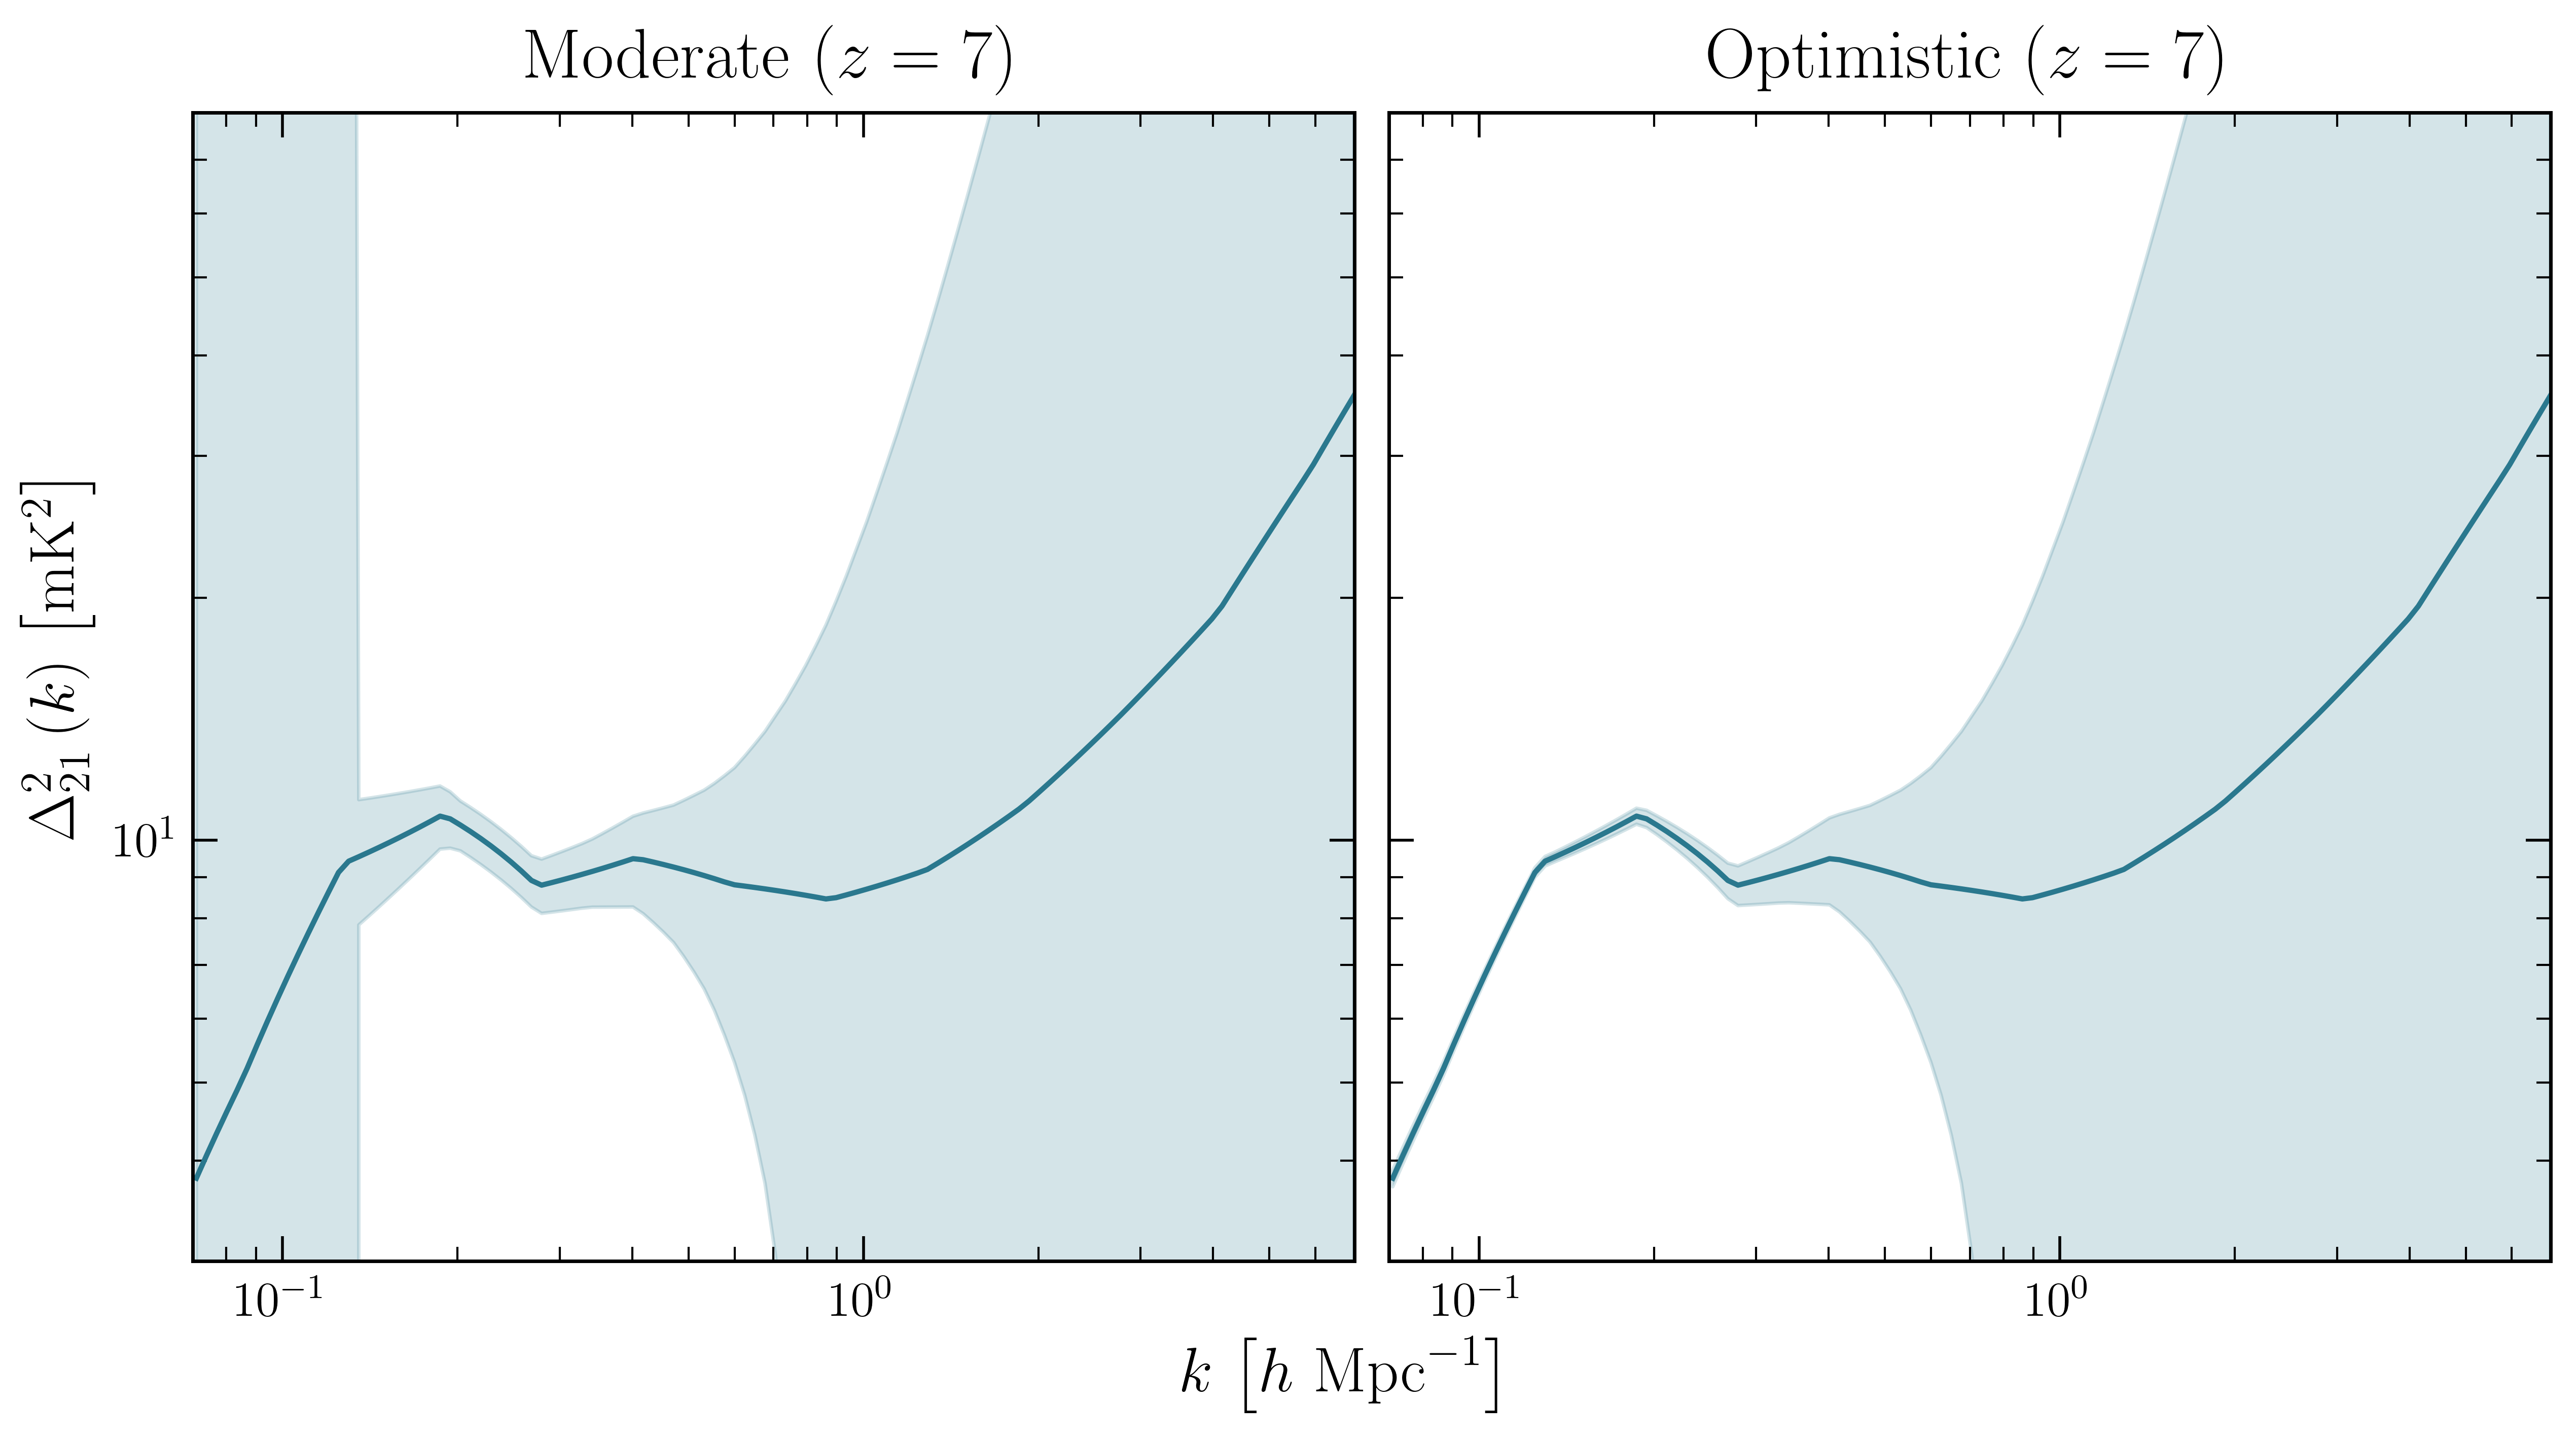
\includegraphics[width=1.0\textwidth]{21cm_errorbars.png}
	\caption[Noise Power Spectrum]{Hello}
	\label{fig:21cm_errors}
\end{figure}

\begin{equation}
    k_{\parallel} \lesssim  \theta \frac{D_{M}\left( z \right) E \left( z \right)}{D_H \left(1 + z\right)} k_{\perp}
\end{equation}

\begin{equation}
    \theta = 1.22 \frac{\lambda}{D}
\end{equation}

Here is an explanation of the wedge

Cross correlation of cosmological 21cm observations with Ly$\alpha$ intensity
mapping surveys have the advantage that 21cm foregrounds do not correlation with
the foregrounds. Because the two do not correlate, no power from the foregrounds
is added to the cross-power spectrum. However, while the foregrounds don't contribute
to the total cross-power spectrum, they do contribute to the overall variance
of the measurement, and therefore the errors.

In the previous section, I calculated the cross-power spectrum for the case where
foreground are completely uncorrelated (don't contribute to the cross-power spectrum
amplitude) and where they did not contribute to the total variance. In this section,
I'll take a more realistic and honest approach to calculating the errors by dealing
with the 21cm foregrounds in two different ways. There are two primary methods
that I chose to deal with the foregrounds: by relying on the fact that the foregrounds
are spectrally smooth and thus confined to an area of the 2D power spectrum known
as the wedge and by assuming some imperfect removal method. Each method has advantages
and disadvantages.

In addition to avoiding 21cm foregrounds by cutting out k-modes that fall within
the wedge, efforts are being made to model 21cm point sources and foregrounds to
directly remove them from the data. This technique is known as foreground subtraction.
While this modeling foregrounds accurately has been shown to be quite difficult,
it gives the added benefit of recovering the foreground modes that fall within
the wedge, increasing the signal to noise of the measurement, assuming perfect (or
near perfect) foreground subtraction.

While outside the scope of this particular project, foreground subtraction could
be a viable method for recovering k-modes afflicated by bright 21cm foregrounds
and potentially allow for higher signal to noise measurements of the cross power
spectrum, given sufficient enough subtraction.

I plan to incorporate a treatment of the foreground subtraction in future works.
Previous works have handled the modeling of the power spectrum due to bright

\begin{equation}
    P_F \left(q, y\right) = \sum_{j} \epsilon_j^2 A_j \left( \frac{l}{2 \pi q} \right)^{n_j} \left( \frac{\nu_p}{\nu_i}\right)^{m_j}
\end{equation}

The total variance on the 21cm-Ly$\alpha$ cross power spectrum measurements would
then be written as:

\begin{equation}
    2 \sigma^2_{21, \rm Ly\alpha} = P^2_{21, \rm Ly\alpha} +
      \left(P_{21} + P_{F} + \sigma_{21} \right) \left( P_{\rm Ly\alpha} + \sigma_{\rm Ly\alpha}\right)
\end{equation}
